\documentclass[12pt]{article}

% Package lists
\usepackage{pythonhighlight}
\usepackage{solarized-dark}
\usepackage{geometry}
\usepackage{graphicx}

% Configurations
\geometry{margin=1cm, bottom=2cm}

\begin{document}
  \title{Report Lab 6}
  \author{Nguyen Tien Duc - ITITIU18029}
  \maketitle
  \part*{1/ Newton's interpolating polynomial}
    \section*{Code}
      \inputpython{Newton.py}{0}{111}
    \section*{Running}
      \begin{center}
        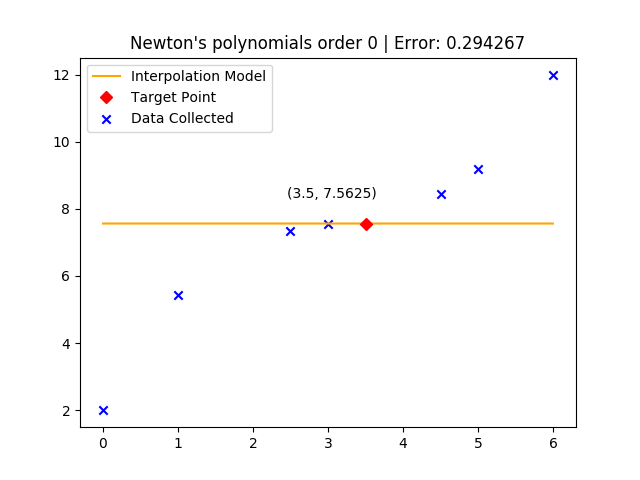
\includegraphics{Order0.png}
        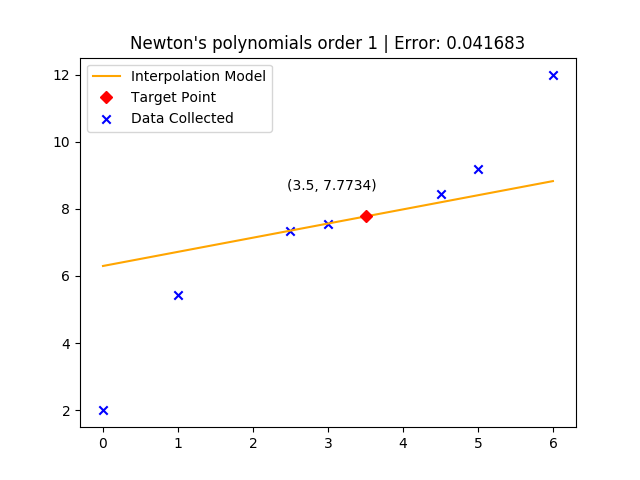
\includegraphics{Order1.png}
        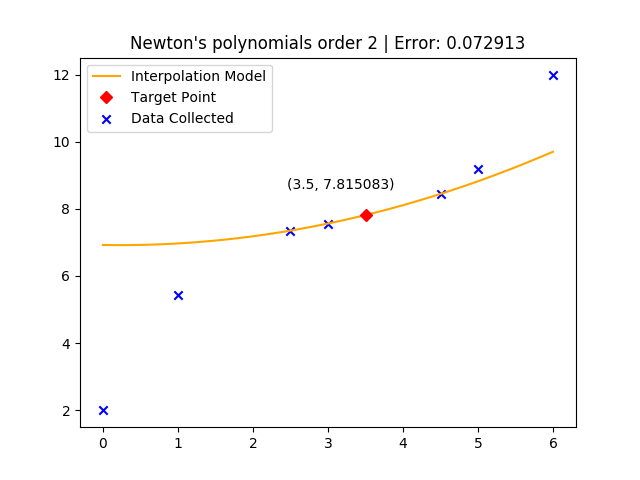
\includegraphics{Order2.png}
        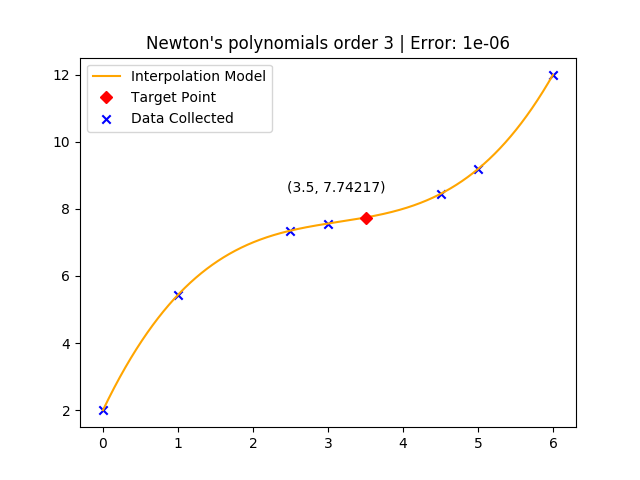
\includegraphics{Order3.png}
        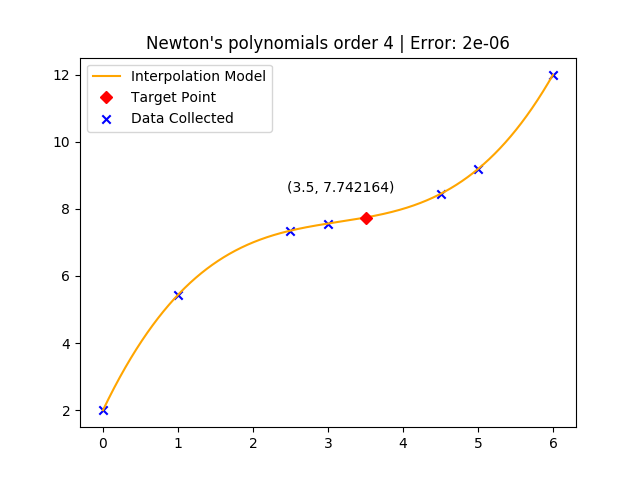
\includegraphics{Order4.png}
        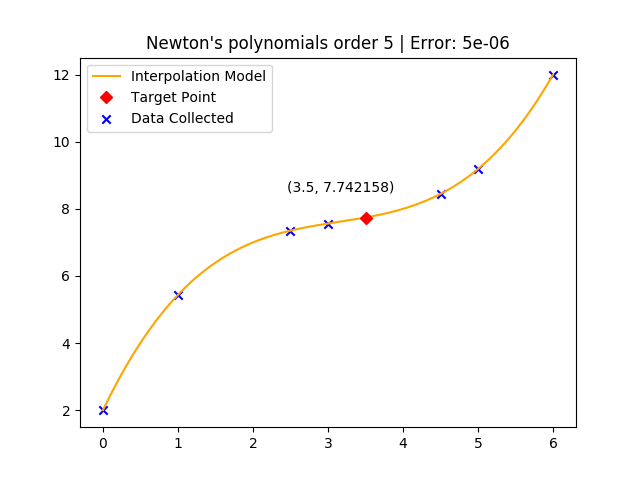
\includegraphics{Order5.png}
        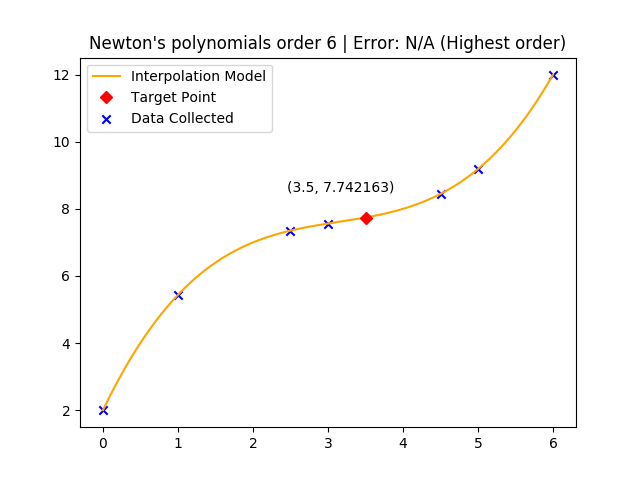
\includegraphics{Order6.png}
      \end{center}
  \part*{2/ Conclusion}
  Through developing the algorithm to find interpolation model in various orders using Newton's interpolating polynomials, things that I learned are:
    \begin{itemize}
      \item The higher the order, the better fit the polynomials model, this is backed by the decrease in truncation error as the order increases.
      \item The lower, not maximum order can still give a fairly accurate estimation given that we choose the data sets with the least squared error.
      In this case, starting from \(3^{th}\) order polynomials the truncation error has already been \(10^{-6}\), which is small enough to ignore and consider the model accurate.
      \item Newton's interpolating polynomials is harder to develop as an algorithm compared to Lagrange's interpolating polynomials.
    \end{itemize}
  \end{document}